\section{Introduction}
\label{sec:intro}

Supercompilation is a semantics-driven program optimisation technique that can automatically deforest intermediate data structures, fuse composed functions, and discover recursive schemes. It works by symbolically evaluating programs (driving), analyzing cases on unknown values (splitting), and recognising repeated configurations (folding). Despite decades of development for first-order and simply-typed languages, supercompilation lacks a proof-theoretic foundation for \emph{dependently typed} languages. In such languages, types depend on terms, contexts evolve during evaluation, and transformations must preserve both typing and observational equivalence.

This paper proposes such a foundation: \emph{every successful supercompilation run yields a valid cyclic proof} in a focused sequent calculus. Driving steps are invertible (asynchronous) sequent rules. Case-splitting on neutral scrutinees is a synchronous choice rule. Memoisation (folding) corresponds to cyclic backlinks that close proof goals by referencing previously-seen vertices. The trace condition that ensures soundness of cyclic proofs matches the termination discipline that justifies folding.

The correspondence is directional: every total supercompilation (one that passes the trace check) constructs a ranked cyclic proof; the converse does not hold — not every cyclic proof can be obtained by supercompilation, and potentially non-terminating programs may yield pre-proofs that fail the trace condition.

While prior work includes Herbelin-style focused calculi for CoC, cyclic proof systems for first-order logic, and informal correspondences between SC operations and proof rules, this is the first to combine focusing, cyclic proof structure, and supercompilation in a dependently typed setting. The combination yields a principled correctness proof (CIU equivalence, mechanised using only functional extensionality) that no prior SC verification framework achieves — Krustev's mechanised SC correctness handles a first-order language; we extend this to CoC with inductives.

A central insight is that \emph{induction principles are discovered post-hoc from the cycle structure}: rather than choosing an induction scheme at the outset of a proof, the cycle formed by backlinks \emph{is} the induction principle, read off from the completed proof graph. This is particularly valuable in dependent types, where type indices containing computations (e.g., $\mathsf{Vec}\;A\;(\mathsf{length}\;(\mathsf{map}\;f\;v))$) must be normalised before rewriting, and the induction scheme must simultaneously simplify the index and prove the property.

This correspondence is not merely a representation change---it has explanatory power.
The trace condition explains \emph{why} folding is sound (every cycle contains a progress event);
the cyclic structure explains \emph{where} recursion comes from (backlinks are discovered during search);
and the CIU equivalence theorem explains \emph{what} correctness means for the residual program (indistinguishable from the source under all observations).

Beyond providing a correctness proof, this perspective reveals supercompilation as a point in a broader design space for proof-directed program transformation. The evaluation strategy determines which rules are invertible; generalisation and back-linking correspond to cut and identity in the sequent calculus; and the strength of the trace condition governs the class of recursive programs handled. Each dimension can be independently varied---call-by-value driving, richer generalisation heuristics, stronger trace conditions---while the core soundness argument remains modular.

\paragraph{Contributions.}
\begin{itemize}[leftmargin=*]
\item A focused cyclic sequent calculus designed to mirror supercompilation operations (Section~\ref{sec:focused}).
\item A precise correspondence between drive/split/fold/generalise and local sequent inference steps, mechanised in Rocq (Section~\ref{sec:equiv}).
\item A four-claim pipeline mechanised using only functional extensionality: pre-proof construction, budget trace cyclic proof, CIU soundness, and example validation (Section~\ref{sec:equiv}).
\item A proof-theoretic account of post-hoc induction discovery via cyclic proofs, with a dependent-type motivation (Section~\ref{sec:thesis:cyclic}).
\end{itemize}

\paragraph{Outline.}
Section~\ref{sec:thesis:pipeline} states the four-claim pipeline.
Sections~\ref{sec:calculus}--\ref{sec:focused} define the source calculus and the focused cyclic sequent system.
Section~\ref{sec:sc-as-search} presents the operational dictionary.
Section~\ref{sec:related} discusses related work, and Section~\ref{sec:equiv} gives the formal results.
The mechanisation is described in the appendix.

\subsection{Main result pipeline}
\label{sec:thesis:pipeline}

\begin{center}
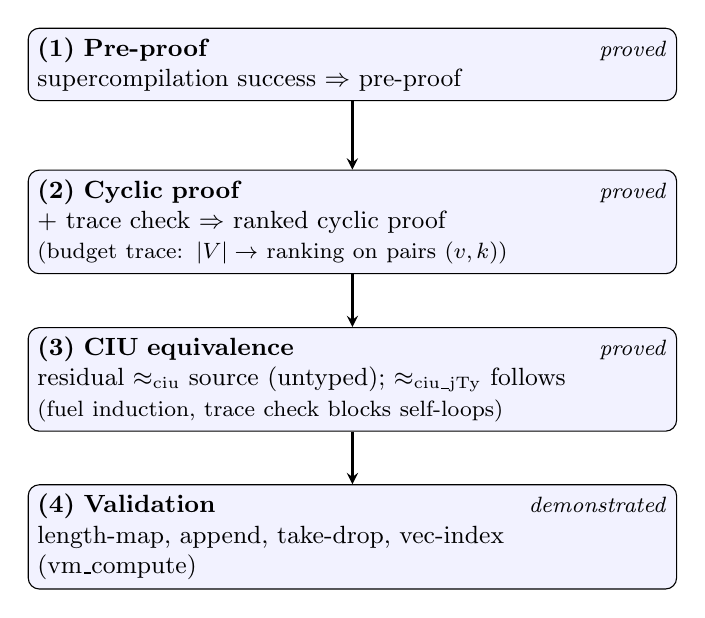
\begin{tikzpicture}[
  node distance=2cm,
  box/.style={rectangle,draw,rounded corners,text width=8cm,align=left,font=\small,fill=blue!5},
  arrow/.style={->,>=stealth,thick}
]
\node[box] (p1) {\textbf{(1) Pre-proof} \hfill {\footnotesize\textit{proved}} \\
  supercompilation success $\Rightarrow$ pre-proof};
\node[box,below of=p1] (p2) {\textbf{(2) Cyclic proof} \hfill {\footnotesize\textit{proved}} \\
  + trace check $\Rightarrow$ ranked cyclic proof \\
  {\footnotesize (budget trace: $|V| \to$ ranking on pairs $(v,k)$)}};
\node[box,below of=p2] (p3) {\textbf{(3) CIU equivalence} \hfill {\footnotesize\textit{proved}} \\
  residual $\approx_{\mathrm{ciu}}$ source (untyped); $\approx_{\mathrm{ciu\_jTy}}$ follows \\
  {\footnotesize (fuel induction, trace check blocks self-loops)}};
\node[box,below of=p3] (p4) {\textbf{(4) Validation} \hfill {\footnotesize\textit{demonstrated}} \\
  length-map, append, take-drop, vec-index (vm\_compute)};

\draw[arrow] (p1) -- (p2);
\draw[arrow] (p2) -- (p3);
\draw[arrow] (p3) -- (p4);
\end{tikzpicture}
\end{center}

The four claims form a dependency chain: each tier builds on the previous. All are mechanized in Rocq using only functional extensionality.

\paragraph{Claim 1: Supercompilation yields a pre-proof.}
When the supercompiler succeeds on a well-typed input, the resulting configuration graph directly forms a \emph{rooted pre-proof}.
Every vertex satisfies its local sequent rule and each edge is justified by the appropriate correspondence (Section~\ref{sec:overview}).
This claim is mechanized in Rocq; see Section~\ref{sec:equiv} (Theorem~\ref{thm:pre-proof}).

\paragraph{Claim 2: Termination yields a cyclic proof.}
A pre-proof becomes a \emph{cyclic proof} when it additionally satisfies a global progress condition: every cycle must contain at least one progress edge (a case-split on a neutral scrutinee), and there exists a well-founded ranking that strictly decreases along progress edges.
The supercompiler enforces this via a trace-condition check during graph construction.
We prove this by constructing a budget-instrumented trace graph: vertices are lifted to pairs $(v,k)$ where $k \in [0, B]$ is a budget counter consumed on progress edges and preserved on non-progress edges.
The resulting trace graph is acyclic, yielding a full $\mathsf{ranking\_condition}$ with rank $\lambda(v,k).\,k$.
This claim is mechanized; see Section~\ref{sec:equiv} (Theorem~\ref{thm:cyclic-proof}).

\paragraph{Claim 3: CIU equivalence.}
The ultimate soundness guarantee is \emph{contextual equivalence} (CIU): the program read off from a valid cyclic proof should be observationally indistinguishable from the original source program under all closing substitutions.
This claim is mechanized by fuel induction; the trace condition prevents self-loops that would introduce non-termination.
See Section~\ref{sec:equiv} (Theorem~\ref{thm:ciu}).

\paragraph{Claim 4: The pipeline obtains for our examples.}
The framework is validated on a suite of standard supercompilation examples (length-map fusion, append length normalisation, take-drop, etc.).
For each example, the supercompiler produces a residual, and computational equality with the expected result is verified by Rocq's $\mathtt{vm\_compute}$.
See Section~\ref{sec:equiv} (Proposition~\ref{prop:examples}) and Section~\ref{sec:example} for a detailed walkthrough.

\subsection{Why focusing matters}

In Andreoli's focusing calculus~\cite{andreoli-1992-logic-programming}, formulas are classified as \emph{positive} or \emph{negative}, and proof search alternates between an \emph{asynchronous phase} (where all invertible rules are applied eagerly) and a \emph{synchronous phase} (where a formula is selected and its non-invertible rules explored). The central theorem is completeness: the focused proof search strategy does not lose provability.

We use ``focusing'' in this operational sense, without defining explicit polarity judgments or phase transitions. A sequent rule is \emph{invertible} if the conclusion implies the premises---i.e., applying the rule eagerly never makes an otherwise provable goal unprovable. Our driving rules ($\beta$/$\iota$/$\delta$) are invertible: each is a single step of the CBN operational semantics, and we prove \texttt{step\_ciu} (CIU.v) that every such step preserves CIU equivalence in both directions ($t' \approx_{\mathrm{ciu}} t$). Case-splitting on neutral scrutinees is non-invertible: choosing the wrong branch can lead to a dead end, so it is a genuine choice point. Concretely, $[x \mid \mathsf{nil}\to 0;\; \mathsf{cons}\to 1]$ with $x$ neutral has CIU source $t$, but the nil-only residual $0$ is not CIU-equivalent: for $x\mapsto\mathsf{cons}\;0\;\mathsf{nil}$, the source evaluates to $1$ while the residual evaluates to $0$ (proved as \texttt{split\_rule\_non\_invertible}, SplitNonInvertible.v). The synchronous phase must therefore explore all branches. Generalisation and folding correspond to cut and identity, respectively---they are synchronous decisions about \emph{which} cut formula to introduce or \emph{which} previous vertex to fold against.

The supercompiler's operational discipline---drive eagerly until stuck, then split or fold---thus instantiates a focused proof search strategy. The completeness of this strategy (that it does not lose programs that could be supercompiled by a different interleaving) is not proved here and is deferred to future work.

\subsection{Why cyclic proofs matter: post-hoc induction}
\label{sec:thesis:cyclic}

In traditional induction, the scheme must be chosen upfront. Cyclic proofs reverse this: begin with the goal, drive and split following the term structure, and form backlinks when goals match previous vertices. The cycle structure \emph{is} the induction principle, read off from the completed graph. The trace condition ensures soundness via structural descent through progress events.

This is particularly valuable in dependent types. Consider $\mathsf{Vec}\;A\;(\mathsf{length}\;(\mathsf{map}\;f\;v))$: the type index contains a computation that must be normalised before rewriting. A traditional proof must choose an induction scheme that simultaneously normalises the index and proves the property. Cyclic proofs avoid this: driving normalises the index during search, and when a fold-back is discovered, the index equality is already reduced to definitional form.

\paragraph{What becomes difficult without this.} In a traditional induction-first framework, proving $\mathsf{Vec}\;A\;(\mathsf{length}\;(\mathsf{map}\;f\;v)) \equiv \mathsf{Vec}\;A\;(\mathsf{length}\;v)$ requires the user to apply the induction hypothesis for $\mathsf{length}\;(\mathsf{map}\;f\;v)$ \emph{inside} the type index, then rewrite. The cyclic approach decouples index normalisation from property proof: driving reduces $\mathsf{length}\;(\mathsf{map}\;f\;v)$ to $\mathsf{length}\;v$ via deforestation during proof search, and the fold recognises the resulting config as a backlink. The induction principle emerges from the completed graph rather than being prescribed. Our mechanised examples include vector-index normalisation where supercompilation reduces the index automatically.
